\section{Modeling Power and Performance}
\label{sec:HBN}


\subsection{Introduction to Probabilistic Graphical Models}
We present an introduction to graphical models in general before we
delve into the details of \SYSTEMLEO{} specifically. Directed graphical
models (or Bayesian networks) are a type of graphical model capturing
dependence between random variables.  Each node in these models
denotes a random variable and the edges denote a conditional
dependence among the connecting nodes. The nodes which have no edges
connecting them are conditionally independent.  By convention shaded
nodes denote an observed variable (\ie one whose value is known),
whereas the unshaded ones denote an unobserved variable. In
\figref[a]{fig:BN}, variables A and B are dependent on C.  If C is
observed, A and B would be independent in \figref[b]{fig:BN}.


\begin{figure}
\begin{center}
	 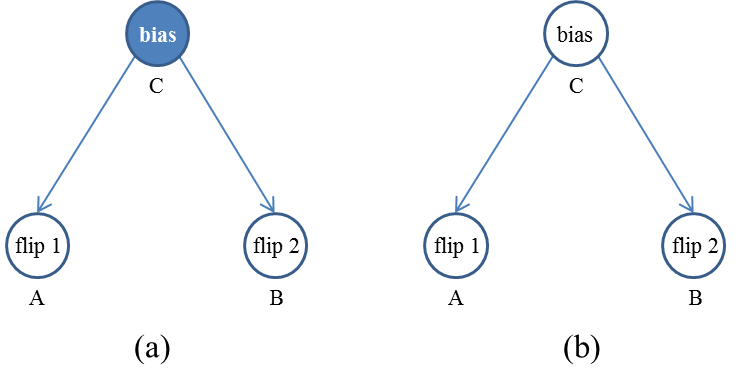
\includegraphics[width=0.45\textwidth]{BayesianModel.png}
\end{center}
\vspace{-0.35em}
\caption{Conditional dependence in Bayesian Model.}
\label{fig:BN}
\end{figure}

The dependence structure in Bayesian networks can be understood using
a coin flipping example with a biased coin.  Suppose A represents the
outcome of the first coin flip, B represents that of second coin flip
and C represents the coin's bias.  Suppose we know this bias is
$P(Heads) = 0.7$, then both the flips are independent --- irrespective
of the first flip the second flip gives \textit{heads} with
probability $0.7$. If the bias is unknown, however, then the value of
$B$ is conditionally dependent on $A$.  Thus, knowing that $A = Heads$
increases belief that the bias is towards \textit{Heads} -- that $C >
0.5$.  Therefore, the probability that the second coin flip gives
\textit{Heads} (\ie $B = Heads$) increases.

\SYSTEMLEO{} exploits this conditional dependence in the presence of
hidden, or unobserved, random variables.  \SYSTEMLEO{} models the
performance and power consumption of every system configuration as a
random variable drawn from a Gaussian probability distribution with
unknown mean and standard deviation.  \emph{Therefore, previously
  observed applications will condition \SYSTEMLEO{}'s estimations of the
  performance and power for new, unobserved applications.}  \PUNT{This
conditional dependence is the key mechanism by which \SYSTEMLEO{} quickly
realizes that \texttt{Kmeans} (from the example section) does not scale past 8
cores.}

\begin{figure*}
\begin{center}
 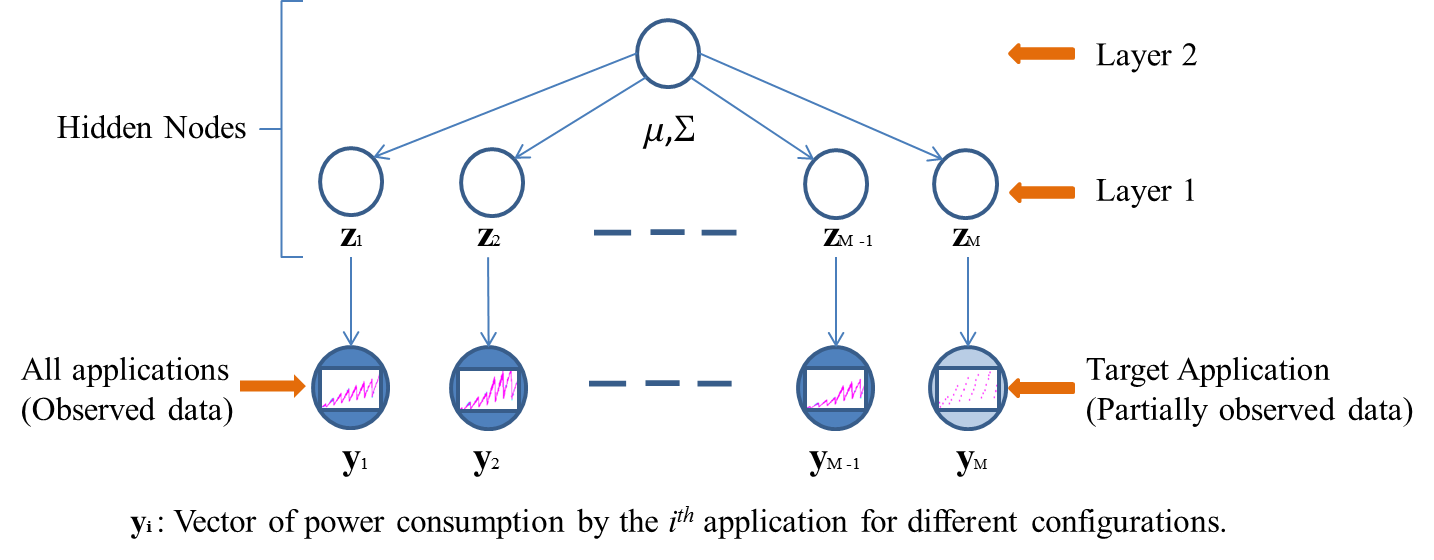
\includegraphics[width=0.85\textwidth]{HierarchicalModel.png}
\vspace{-0.35em}
\caption{Hierarchical Bayesian Model.}
\label{fig:HBN}
\end{center}
\end{figure*}


\subsection{Hierarchical Bayesian Model}
Hierarchical Bayesian Models are slightly more complex Bayesian
networks, usually with more than one layer of hidden nodes
representing unobserved variables. \SYSTEMLEO{} utilizes these hidden
nodes to improve its estimates for a new application using prior
observations from other applications. The intuition is that
\textit{knowing about one application should help in producing better predictors for other applications}. In our examples, learning about one
biased coin flip should tell us something about another.  Similarly,
learning about another application that scales up to 8 cores should
tell us something about Kmeans. \SYSTEMLEO{} utilizes this conditional
dependence in the problem of performance and power prediction for an
application using other applications. \SYSTEMLEO{}'s model is explained
in the figure \figref{fig:HBN},

Suppose we have $n = |\mathcal{C}|$ configurations in our system.  We
have a \textit{target application} whose energy we wish to minimize,
while meeting a performance requirement (as in \eqref{eq:controller}).
Additionally, we have a set of $M-1$ applications whose performance
and power are known (as they have been measured offline).

%\TODO{Consider replacing y with p to be consistent with prior section.}
  We will illustrate how \SYSTEMLEO{} estimates power as a
function of system configuration. The identical process is used to
estimate performance.  Let the vector $\y_i \in \R^{n}$ represent the
power estimate of application $i$ in all $n$ configurations of the
system; \ie the $c$th component of $\y_i$ is the power for application
$i$ in configuration $c$ (or $\y_i[c] = p_c$).  Also, let $\{\y_i\}_{i =1}^M$ be the shorthand for the power estimates for all applications.  Without loss of generality, we assume that the first $M-1$
columns, \ie $\{\y_i\}_{i =1}^{M-1}$ represent the data for those
applications whose power consumption is known (this data is collected
offline).  The $M$th column, $\y_M$ represents the power consumption
for the new, unknown application.  We have some small number of
observations for this application.  Specifically, for the $M$th application we have observed
configurations belonging to the set $\Omega_M$ where $|\Omega_M| \ll
n$; \ie we have a very small number of observations for this
application.  Our objective is to estimate the power for application
$M$ for all configurations that we have not observed.
The model is described in terms of statistical equations below,

\begin{equation}
\begin{aligned}
\y_i \vert \z_i  &\sim N( \z_i, \sigma^2 \I),\\
\z_i \vert \mu,\Sigma &\sim N(\mu, \Sigma),\\
\mu, \Sigma &\sim N(\mu_0,\Sigma / \pi)IW(\Sigma | \nu, \Psi),
\end{aligned}
\label{eq:HBN}
\end{equation}

where $\y_i \in \R^n, \;
\z_i \in \R^n, \;
\mu \in \R^{n}, \;
\Sigma \in \R^{n\times n}$. It describes that the power (denoted by $\y_i$) for each of the $i^{th}$ application,  is drawn from multivariate-Gaussian distribution with mean $\z_i$ and a diagonal covariance matrix $\sigma^2\I$. Similarly, $\z_i$ is from multivariate-Gaussian distribution with mean $\mu$ and covariance $\Sigma$. And, $\mu$ and $\Sigma$ are jointly drawn from normal-inverse-Wishart distribution with parameters  $\mu_0, \pi,\Psi, \nu$. The parameters for our model are $\mu,\Sigma$, whereas,  $\mu_0, \pi,\Psi, \nu$ are the hyper-parameters, which we set as $\mu_0 = 0, \pi = 1,\Psi = \I, \nu = 1$.

The first layer in this model as described in \figref{fig:HBN}, is the filtration layer and accounts for the measurement error for each application. Interestingly, even if we have just a single measurement of each configuration for each application, this layer plays a crucial role as it creates a shrinkage effect. The shrinkage effect penalizes large variations in the application and essentially help in reducing the risk of the model (See \cite{efron1975data} for  shrinkage effect and \cite{morris1983parametric} for shrinkage in hierarchical models). The second layer on the other hand binds the variable $\z_i$ for each application and
enforces that they are drawn from the same distribution with unknown
mean and covariance. We work with a normal-inverse-Wishart distribution as described in \cite{gelman2013bayesian} as our hyper prior on $\mu, \Sigma$, since this distribution is the conjugate prior for a multivariate Gaussian distribution.
Thus, we essentially have a normal means model at
the first level of our hierarchy for each of the different apps and we
have a Gaussian prior on the parameter of this model. Now, if the mean
$\mu$, covariance $\Sigma$ and noise $\sigma$ were known, $\y_i$ are
conditionally independent given these parameters. Since they are
unknown we have introduced a dependence amongst all the $\y_i$s. This
is a similar situation to our coin flipping example in \figref{fig:BN}, where the value of one coin influences our prediction
about the other coin. $\Sigma$ captures the correlation between different configurations as depicted in \figref{fig:Sigma}.



\begin{comment}
\vspace{-0.35em}
\begin{algorithm}[h]
\caption{\SYSTEMLEO{} algorithm for power estimation}
\begin{algorithmic}[1]
\REQUIRE M $\leftarrow$ Number of applications, n $\leftarrow$ Number of configurations. $\{\y_i\}_{i = 1}^{M}$ $\leftarrow$ Power measurements for M applications. $\Omega_i$  $\leftarrow$ Known indices in $\y_i$. $\Omega$  $\leftarrow$ $ \{\Omega_i\}_{i = 1}^{M}$, $\epsilon \leftarrow \text{Tolerance to control convergence}$.

\STATE Construct indicator matrix $L \in \R^{n x M}$ from $\Omega$. $L_i(j) = 1$ if $j \in \Omega_i$, $L_i(j) = 0$ otherwise.
\STATE Initialize $\theta = \mu, \Sigma,\sigma$ and likelihood $\hat{\textit{L}}_0, \epsilon$.
\STATE Set $\hat{\textit{L}}  = 2\hat{\textit{L}}_0 $.
\REPEAT
	\STATE Expectation step: Compute $C_i$ and $\hat{\z}_i$ using \eqref{eq:conditionals},
	\STATE Maximization step: Compute $\theta = (\mu, \Sigma, \sigma)$ using \eqref{eq:maximization},
	\STATE Calculate likelihood $\hat{\textit{L}}  = \textit{L} \left(\theta  \vert \{ \phi(y_i ) \}^M, \{ \hat{\z}_i\}^M \right)$ using Equation \eqref{eq:likelihood}.
	\STATE Set $\hat{\textit{L}}  = \hat{\textit{L}}_0  $.
\UNTIL{$\frac{\|  \hat{\textit{L}} - \hat{\textit{L}}_0  \|}{\hat{\textit{L}}_0 } > \epsilon$}
\STATE $ \hat{\y}_M = \hat{\z}_M$
\RETURN $ \hat{\y}_M$.
\end{algorithmic}
\label{alg:LEO}
\end{algorithm}
\end{comment}
We use $\theta = \{\mu, \Sigma, \sigma\}$ to denote the unknown
parameters in the model. It can be shown that $\y_M$ is Gaussian given
$\theta$ (See \cite{yu2005learning}). %\TODO{Never say ``it can be shown.''  Always either show it   or have a citation.  Then you just say, $\y_M$ is Gaussian givenm  $\theta$ and cite or refer to your prior derivation.}.
 Thus, the problem boils down to estimating $\theta$.  Maximum-likelihood
estimators are the set of values of the model parameters that
maximizes the likelihood function (or the probability function of the
observed outcomes given the parameter values).  Essentially, the
maximum-likelihood estimates of parameters are those values which most
agree with the model. Suppose $\phi(\y)$ is the set of the observed
entries in vector $\y$. Ideally, we would like to find the maximum
likelihood estimate of the parameter $\theta$ by maximizing the
probability of $\y_M$ conditioned on ${\phi(\y_i)}_{i = 1}^{M}$ and
then use the expectation of $\y_M$ given ${\phi(\y_i)}_{i = 1}^{M}$
and $\hat{\theta}$ and as our estimator for $\y_M$. Due to the presence of latent variables (layer 1 and layer 2 in \figref{fig:HBN}) , we do not have a closed form for $\Pr( \y_M | \{\phi(\y_i)\}_{i = 1}^{M}, \theta )$
and we have to resort to the iterative algorithms like Expectation
Maximization algorithm to solve this problem.


\subsection{Expectation Maximization Algorithm}
\label{sec:EMalg}
The EM (Expectation Maximization) algorithm is a popular approach in
statistics for optimizing over analytically intractable problems.
The EM algorithm switches between two steps: \emph{expectation} (E)
and \emph{maximization} (M) until convergence. During the E step, a
function for the expectation of the log of the likelihood is found
using the current estimate for the parameters.  In the M step, we
compute parameters maximizing the expected log-likelihood found on the
E step. These parameter estimates are then used to determine the
distribution of the latent variables in the next E step.  We have left
out some details of the algebra here, but a more detailed proof on
similar lines can be found here \cite{yu2005learning}.

As described earlier, $\Omega_i$ is the set of observed indices for
$i^{th}$ application. Let $L$ denote the indicator matrix with $L(i,j)
= 1$ if $j \in \Omega_i$
and $0$ otherwise. That is, $L(i,j) = 1$ if we have observed application $i$ in system configuration $j$.  We are using $L_i$ for $L(:,i)$ for $i^{th}$ application for shorter notation. We can write the expectation and covariance for $\z_i$ given $\theta$ as following,

\begin{equation}
\begin{aligned}
\label{eq:expectation}
 \text{Cov}(\z_i) =  \left( \frac{\diag(L_i)}{\sigma^2} +\Sigma^{-1} \right)^{-1} \;\; \text{and} \\
 \E(\z_i) = \hat{\mathbf{C}}_i \left(  \frac{\diag(L_i) \y_i}{\sigma^2} +  \Sigma^{-1} \mu  \right).
 \end{aligned}
\end{equation}

\begin{comment}
\textbf{E step}: We calculate the expected log-likelihood as,
$$Q(\theta) = \E_{\{\z_i\}^M | \{ \phi(\y_i) \}^M, \mu, \Sigma }( -\log (f ( \{ \phi(y_i )  \}^M, \{\z_i\}^M  \vert \theta)f(\mu,\Sigma)  ), $$

The log of the likelihood function is given by,
\begin{equation}
\begin{aligned}
&\textit{L} \left(\theta \vert \{ \phi(y_i ) \}^M, \{ \z_i\}^M \right)
= \log(f \left( \{ \phi(y_i ) \}^M, \{ \z_i\}^M \vert \theta \right)),\\
&=   -\frac{1}{2} \mathlarger{ \sum}_{i = 1}^M [   \z_i' \left( \frac{\diag(L_i)}{\sigma^2} + \Sigma^{-1} \right) \z_i   - 2\left( \frac{y_i' \diag(L_i)}{\sigma^2}+\mu' \Sigma^{-1}  \right)\z_i  \\
&+ \frac{y_i' \diag(L_i) y_i}{\sigma^2}  + \mu'\Sigma^{-1}\mu  ]  - \log \left((\sqrt{2\pi\sigma})^{\| L\|_F^2} (2\pi \det(\Sigma))^\frac{M}{2}\right),\\
 \end{aligned}
 \label{eq:likelihood}
\end{equation}
Thus after some algebraic manipulation we have,
\begin{equation}
\begin{aligned}
\label{eq:estep}
Q(\theta) & = \text{Const} +  \mathlarger{ \sum}_{i = 1}^M   [ \tr \left( \left( \frac{\diag(L_i)}{\sigma^2} + \Sigma^{-1} \right) (\hat{\mathbf{C}}_i + \hat{\z}_i  \hat{\z}_i') \right) \\
&-2\left( \frac{\y_i' \diag(L_i)}{\sigma^2} +\mu' \Sigma^{-1}  \right)\hat{\z}_i   + \frac{\y_i' \diag(L_i) \y_i}{\sigma^2}  \\
&+ \mu'\Sigma^{-1}\mu  + \frac{ \| L\|_F^2}{M} \log(\sigma^2) + \log(\det(\Sigma)) ] \\ &+\log(\det(\Sigma))+\pi\mu'\Sigma^{-1}\mu+\tr(\Sigma^{-1}) ,
 \end{aligned}
\end{equation}
\end{comment}

We use $\hat{\mathbf{C}}_i$ as shorthand for  $\text{Cov}(\z_i)$ and $\hat{\z}_i$ denotes  $\E(\z_i)$. Later, we maximize log-likelihood w.r.t. $\theta$ and
taking derivative w.r.t. $\Sigma,\sigma \text{ and }\mu$ and setting them to 0 gives,
\begin{equation}
\label{eq:maximization}
\begin{aligned}
&\mu = \frac{1}{M +\pi} \sum_{i = 1}^M \hat{\z}_i,  \\
&  \Sigma = \frac{1}{M+1} \left(\sum_{i = 1}^{M}\hat{\mathbf{C}}_i + (\hat{\z}_i -\mu)(\hat{\z}_i -\mu)'\right) +\pi\mu\mu' +\I,\\
& \sigma^2 = \frac{1}{\|L\|_F^2} \sum_{i = 1}^{M}  \tr\left(\diag(L_i)(\hat{\mathbf{C}}_i' + (\hat{\z}_i - \y_i)(\hat{\z}_i - \y_i)' )\right),\\
 \end{aligned}
\end{equation}

\PUNT{
The estimation algorithm would repeat \eqref{} and  \eqref{} alternately until convergence.

Algorithm \ref{alg:LEO} summarizes how \SYSTEMLEO{} applies the E and M
steps to use prior observations to estimate values for unseen
configurations.

The algorithm alternates between the E step  and the M
step until convergence and the convergence criterion checks if the
relative likelihood (measured using Equation \eqref{eq:likelihood}) is
sufficiently small.
}

\SYSTEMLEO{} iterates over the E step (equation \eqref{eq:expectation})
and M step (equation \eqref{eq:maximization}) until convergence to
obtain the estimated parameters $\theta$. Then, conditioned on those
values of the parameters, \SYSTEMLEO{} sets $\y_M$ as $\E(\z_M | \theta)$
given by \eqref{eq:expectation}. \SYSTEMLEO{} uses the same algorithm to
estimate performance as well.

Given performance and power estimates, the energy minimization problem
can be solved using existing convex optimization techniques
\cite{PTRADE,ControlWare,Agilos,Heartbeats2}.  \SYSTEMLEO{} simply first
take the estimates, then finds the set of configurations that
represent Pareto-optimal performance and power tradeoffs, and finally
walks along the convex hull of this optimal tradeoff space until the
performance goal is reached.  The configuration representing this this
point in the Pareto-optimal space is the desired tradeoff.

\subsection{Example}
We illustrate how \SYSTEMLEO{} can be applied to our running example of
\texttt{Kmeans} from \Secref{sec:example}. We have 32 configurations
(hence $n=32$) corresponding to cores. We also have 24 other
applications (hence $M = 25$) with all the data for different
configurations collected offline and denoted by
$\{\y_i\}_{i=1}^{M-1}$; $\y_M$ denotes the power data for
\texttt{Kmeans}. Referring to \figref{fig:HBN}, \texttt{Kmeans} is the
final node, labeled ``Target Application,'' whereas the rest of the
applications would be the remaining nodes in any order. \SYSTEMLEO{}
estimates $\z_M$, the node above $\y_M$ in \figref{fig:HBN}, which is
an unbiased estimator for $\y_M$. \SYSTEMLEO{} collects data $\y_M$ for 6
different configurations (5, 10, $\cdots$, 30 cores). Hence, $\Omega_M
= \{5, 10, \cdots, 30 \}$ and $\y_M[j]$ is known iff $j \in \Omega_M$.
Also, $L_i$ or $L(:,i)$ is an all one vector of length $n$ if $i \neq
M$ and $L(j,i) = 1 \text{ if } j \in \Omega_M$ and $L(j,i) = 0$
otherwise.

Now, we describe the main steps of \SYSTEMLEO{}. The algorithm starts by
setting some initialization for the parameter $\theta = \{\mu, \Sigma,
\sigma\}$ and then evaluates equation \eqref{eq:expectation} for each
$i$th and later uses these values of $\hat{\z}_i$ and $\hat{C}_i$ to
evaluate equation \eqref{eq:maximization}, which is fed back to
expectation \eqref{eq:expectation} and so on. This alternating step
between equation \eqref{eq:expectation} and \eqref{eq:maximization}
runs until the algorithm converges. The algorithm uses $\hat{\z}_M$ as
the estimate of \texttt{Kmeans} power (\ie $p_c = \hat{\z}_M[c],
\forall c \in \mathcal{C}$ in equation \eqref{eq:controller}).
Similarly, \SYSTEMLEO{} estimates the performance $r_c$. After the
estimation step the linear program in equation \eqref{eq:controller}
is solved to obtain the best configuration.

\subsection{Discussion}

\begin{figure}
\begin{center}
\begin{tabular}[h]{cc}\hspace*{-15pt}
	 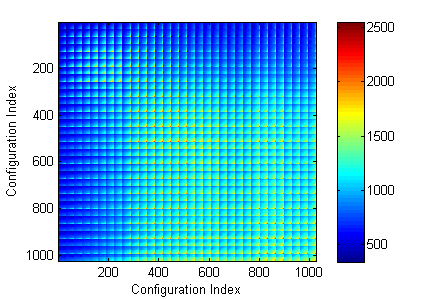
\includegraphics[width=0.45\textwidth]{Sigma.png}
\end{tabular}
\end{center}
\vspace{-1.46em}
\caption{A illustrative example of covariance $\Sigma$  between different configurations, in equation \eqref{eq:HBN}}
\label{fig:Sigma}
\end{figure}

The key to \SYSTEMLEO{} is that it does not assume any parametric
function to describe how the power varies along the underlying
configuration knobs such as cores, memory controllers or speed
settings. The upside of this representation is that \SYSTEMLEO{} captures
a much wider variety of applications, whereas the downside is a higher
computational load. \SYSTEMLEO{} finds covariance in the configurations
and exploits these relationships to estimate the data for each of the
configurations (See \figref{fig:Sigma}). We want to again point out
how our modeling of the problem is markedly different from some of
the previous approaches (such as \cite{deng2012coscale}), which assume
that power and performance are convex functions of the configuration
knobs and employ algorithms similar to gradient descent to find the
optimal configuration. While such methods work well for most
applications, it may not be suitable for more complicated
applications. \emph{In contrast, \SYSTEMLEO{} assumes that there will be
  many local minima and maxima in the functions mapping system
  configuration to power and performance -- \SYSTEMLEO{} is designed to be
  robust to the presence of local extrema, but this property is achieved at a cost of
  higher computational complexity.}

We describe some of the properties of \SYSTEMLEO{}. The EM algorithm's
convergence is dependent on the initial model
\cite{wu1983convergence}.  We can initialize the algorithm randomly.
Empirically, however, we observe that the initialization of $\mu$ with
the estimates from the online or offline approaches (given in
\Secref{sec:poc}) improves \SYSTEMLEO{}'s accuracy.  Experimentally we
have observed that the algorithm converges quickly for our benchmark
sets, generally requiring 3-4 iterations to reach the desired
accuracy. We discuss the overhead of \SYSTEMLEO{} further in
\Secref{sec:experiment:overhead}. \PUNT{In our experiments we also
  normalize the applications so that they are on the same scale, it
  helps in improving the overall accuracies.}
